\subsubsection{\textit{Minimax}}
  \textit{Minimax}\cite{noauthor_minimax_nodate, fan_minimax_1953} (\textit{MM}) es un 
  algoritmo de decisión utilizado en múltiples ámbitos para minimizar la pérdida posible para 
  el \enquote{peor caso} (\textit{maximum loss}). 
  Se formuló originalmente para juegos de suma cero de \(n\) jugadores, pero se ha extendido a
  juegos más complejos y a problemas de decisión con incertidumbre.

  \begin{definition}[\textbf{Valor \textit{Maximin}}]
    El valor \textit{maximin} de un estado del juego es la máxima cantidad de recursos que puede 
    obtener un jugador, sin conocer las jugadas de su oponente.

    Formalmente:
    \[
      \underline{v_{i}} = \max_{a_{i}}\min_{a_{-i}}v_{i}(a_{i},a_{-i})
    \]
    Donde:
    \begin{itemize}
      \item \(i\) es el índice del jugador actual.
      \item \(-i\) representa a todos los jugadores oponentes.
      \item \(a_i\) es la jugada del jugador \(i\).
      \item \(a_{-i}\) son las jugadas de todos los oponentes.
      \item \(v_i\) es la función de evaluación del estado del juego en el turno del jugador 
        \(i\).
    \end{itemize}
  \end{definition}

  \begin{definition}[\textbf{Valor \textit{Minimax}}]
    El valor \textit{minimax} de un estado del juego es la mínima cantidad de recursos que un 
    oponente puede forzar al jugador a perder, sin saber las jugadas del jugador.
    
    Formalmente:
    \[
      \overline{v_{i}} = 
        \min_{a_{-i}}\max_{a_{i}}{v_{i}(a_{i}, a_{-i})}
    \]
  \end{definition}

  \begin{definition}
    Se define la función \(MM\) para un estado del juego \(s\) como:
    \[
      MM_i(s) = \begin{cases}
        v_i(s) & \text{si } s = F  \\
        \underline{v_{i}}(s) & \text{si es el turno del jugador } i \\
        \overline{v_{i}}(s) & \text{si es el turno del oponente } -i
      \end{cases}  
    \]
    Con \(F\) representando el estado final del juego.
  \end{definition}

  \begin{definition}[\textbf{Algoritmo \textit{Minimax}}]
    Sea \texttt{t} un árbol de estados del juego, donde cada nodo del árbol es un estado del juego
    evaluado con la función de evaluación \(v_i\), y donde cada arco del árbol es una jugada de un
    jugador (para simplificar diremos que cada jugada representa un turno y que los jugadores 
    toman turnos alternados, primero \(i\) y luego \(-i\)).
    Luego, cada nodo tendrá tantos hijos como jugadas pueda realizar cada jugador en su turno.

    Se define el algoritmo \textit{minimax} para un árbol de estados \texttt{t} como:
    
    \begin{minted}{kotlin}
      fun minimax(t: StateTree, player: Player in [i, -i]): Double =
        if (t.isTerminal()) {
          t.value
        } else if (player == -i)  {
          t.children.maxOf { child -> minimax(child, i) }
        } else {
          t.children.minOf { child -> minimax(child, -i) }
        } 
    \end{minted}
  \end{definition}

  
  \begin{figure}[ht!]
    \centering
    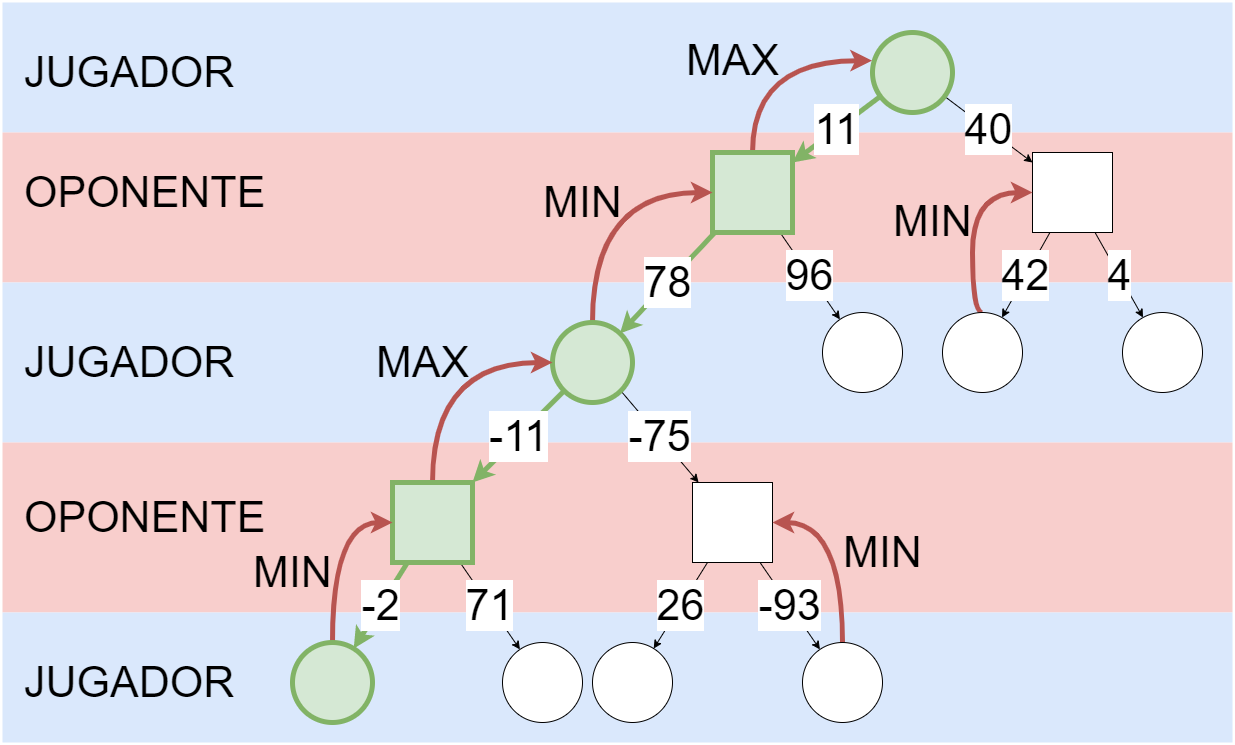
\includegraphics[width=0.6\textwidth]{img/minimax.drawio.png}
    \caption{Árbol de estados de un juego.}
    \label{fig:minimax-tree}
  \end{figure}

  Para entender mejor el algoritmo, considere el árbol de estados de la 
  \cref{fig:minimax-tree}.
  Cada nodo del árbol representa un estado del juego, y cada arco representa una jugada de un 
  jugador.
  Con esto podemos definir una función de evaluación arbitraria donde el valor de cada nodo
  es la suma de puntajes acumulados en el camino que conecta la raíz del árbol con el nodo.
  Aplicando esta función de evaluación al algoritmo \textit{minimax} se toman las decisiones
  indicadas por las flechas rojas en la figura, tomando el mínimo o máximo dependiendo de quién
  sea la jugada.
  Finalmente se escoge la secuencia de jugadas marcadas en verde.